\documentclass[11pt,a4paper]{article}

\usepackage{iftex}
\ifPDFTeX
  \usepackage[T1]{fontenc}
  \usepackage[utf8]{inputenc}
  \usepackage{lmodern}
\else
  \usepackage{fontspec}
  \setmainfont{lmroman10-regular.otf}[BoldFont=lmroman10-bold.otf,
    ItalicFont=lmroman10-italic.otf, BoldItalicFont=lmroman10-bolditalic.otf]
  \setsansfont{lmsans10-regular.otf}[BoldFont=lmsans10-bold.otf,
    ItalicFont=lmsans10-oblique.otf]
  \setmonofont{lmmono10-regular.otf}[ItalicFont=lmmonoslant10-regular.otf]
\fi
\usepackage[margin=2.4cm]{geometry}
\usepackage{amsmath,amssymb,amsthm}
\usepackage{tikz}
\usepackage{tikz-cd}
\usepackage{booktabs}
\usepackage{longtable}
\usepackage{enumitem}
\usepackage{microtype}
\usepackage[hidelinks]{hyperref}

\usetikzlibrary{positioning,arrows.meta,calc,fit,backgrounds}

\theoremstyle{definition}
\newtheorem{defn}{Definition}[section]
\newtheorem{examplex}{Example}[section]
\newtheorem{rmk}{Remark}[section]

\newcommand{\lean}[1]{\textsf{\small #1}}
\newcommand{\Rn}{\mathbb{R}^n}

\title{\textbf{Products}\\[2mm]
\large Lawvere--Schanuel's first exercise, answered for\\
\emph{Kalkulus I} (MBLK37E) and \emph{Lineáris algebra I} (MBLK15E)}
\author{}
\date{}

\begin{document}
\maketitle

\begin{abstract}
Exercise~1 of Lawvere and Schanuel's \emph{Conceptual Mathematics} asks the reader to find
products ``in life'' and in other circumstances.  This note answers it three times over.
Section~\ref{sec:test} states the one test that decides whether something is a product.
Section~\ref{sec:life} runs the test on twelve everyday situations.
Section~\ref{sec:syllabi} goes through the two \emph{Tárgytematika} documents item by item
and sorts every occurrence of the word \emph{szorzat} into the two possible meanings ---
a \emph{product object} (a pair) and a \emph{multiplication map} (a map \emph{out of} a
pair).  Section~\ref{sec:atlas} does the same for the exercise sheets
\texttt{kalkulus\_gyakorlo.pdf}.  Section~\ref{sec:exam} turns all of it into a protocol
for a timed exam.  Every mathematical claim made here is stated and proved in
\texttt{RequestProject/ProductOverlap.lean}; the Lean name is printed in the margin of the
claim, e.g.\ \lean{type\_isProduct}.
\end{abstract}

\tableofcontents

\section{The one test}\label{sec:test}

\begin{defn}[Lawvere--Schanuel]\label{def:prod}
Let $X$ and $Y$ be objects of a category.  An object $P$ together with two maps
$p:P\to X$ and $q:P\to Y$ is a \emph{product} of $X$ and $Y$ if for every object $T$ and
every pair of maps $f:T\to X$, $g:T\to Y$ there is \emph{exactly one} map
$\langle f,g\rangle : T\to P$ with
\[
  \langle f,g\rangle ; p = f, \qquad \langle f,g\rangle ; q = g .
\]
\end{defn}

\begin{center}
\begin{tikzcd}[column sep=6em,row sep=large]
 & T \arrow[dl,swap,"f"] \arrow[d,dashed,"{\exists!\ \langle f,g\rangle}"] \arrow[dr,"g"] & \\
X & P \arrow[l,"p"] \arrow[r,swap,"q"] & Y
\end{tikzcd}
\end{center}

\noindent\emph{Lean:} \lean{ProductOverlap.IsProduct}.

The definition never mentions elements.  It says: \emph{to give one thing of type $P$ is
the same as to give one thing of type $X$ and one thing of type $Y$}.  That sentence is the
exam-usable form of the test.  Two consequences, both proved once and then reused:

\begin{itemize}[nosep]
\item \textbf{Uniqueness.}  Any two products of the same $X,Y$ are isomorphic by a unique
      isomorphism commuting with the projections --- \lean{IsProduct.unique\_up\_to\_iso}.
      So ``the'' product is legitimate language, and any construction passing the test is
      as good as any other.
\item \textbf{Commutativity for free.}  $(Y\times X,\ \mathrm{snd},\ \mathrm{fst})$ also
      passes the test for $X,Y$, hence $X\times Y\cong Y\times X$ --- \lean{swap\_isProduct},
      \lean{prod\_comm\_iso}.  Choosing the colour first and the size second is the same
      as the other way round.
\end{itemize}

\subsection*{Product object versus multiplication map}

This distinction organises everything below, and is the single most useful thing to carry
into an exam.

\begin{center}
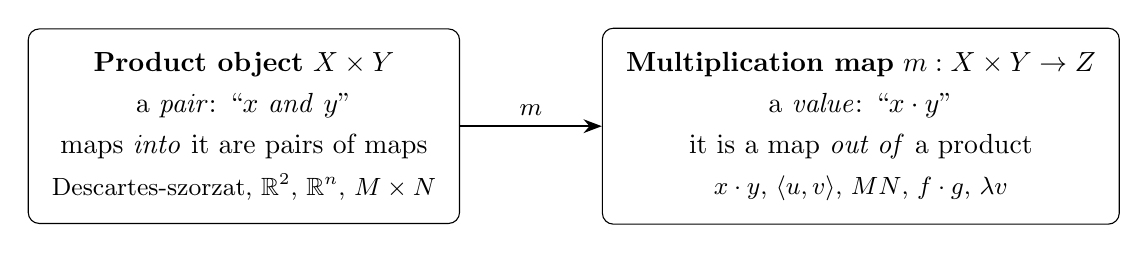
\begin{tikzpicture}[node distance=6mm]
\node[draw,rounded corners,align=center,inner sep=3mm] (a)
  {\textbf{Product object} $X\times Y$\\[1mm]
   a \emph{pair}: ``$x$ \emph{and} $y$''\\[1mm]
   maps \emph{into} it are pairs of maps\\[1mm]
   \small Descartes-szorzat, $\mathbb{R}^2$, $\mathbb{R}^n$, $M\times N$};
\node[draw,rounded corners,align=center,inner sep=3mm,right=18mm of a] (b)
  {\textbf{Multiplication map} $m:X\times Y\to Z$\\[1mm]
   a \emph{value}: ``$x\cdot y$''\\[1mm]
   it is a map \emph{out of} a product\\[1mm]
   \small $x\cdot y$, $\langle u,v\rangle$, $MN$, $f\cdot g$, $\lambda v$};
\draw[-{Stealth},thick] (a) -- node[above,font=\small]{$m$} (b);
\end{tikzpicture}
\end{center}

Both are called \emph{szorzat} in Hungarian and \emph{product} in English, but they are
different kinds of thing: the first is an object, the second an arrow.  A pointwise
product of functions is the composite of both:
\[
  f\cdot g \;=\; m\circ\langle f,g\rangle ,
  \qquad
  \begin{tikzcd}[ampersand replacement=\&,column sep=large]
  \mathbb{R} \arrow[r,"\langle f{,}g\rangle"] \& \mathbb{R}\times\mathbb{R} \arrow[r,"m"] \& \mathbb{R} .
  \end{tikzcd}
\]
Every theorem about products of functions in \emph{Kalkulus I} is obtained by feeding a
property of $\langle f,g\rangle$ (it is continuous/differentiable coordinatewise) into a
property of $m$ (it is continuous, and bilinear).  See
Sections~\ref{sec:syllabi} and \ref{sec:exam}.

\section{Products in life}\label{sec:life}

Run the test of Definition~\ref{def:prod} on each situation: \emph{is specifying one thing
of the whole exactly the same as specifying one thing of each part, with no leftover choice
and no clash?}

\begin{longtable}{@{}p{0.30\textwidth}p{0.30\textwidth}p{0.34\textwidth}@{}}
\toprule
\textbf{Situation} & \textbf{The two projections} & \textbf{Why it passes (or fails)}\\
\midrule
\endhead
A shirt in a shop & colour; size & Choosing a shirt $=$ choosing a colour and a size.
$3$ colours, $2$ sizes, $6$ shirts. \lean{shirts\_card}\\
A square of a chessboard & file (a--h); rank (1--8) & ``e4'' \emph{is} the pair; $64=8\cdot 8$
squares. \lean{card\_prod\_eq\_mul}\\
An appointment & day; time of day & The calendar grid is literally drawn as a rectangle.\\
A point on the screen & $x$ pixel; $y$ pixel & The plane; the projections are the two rulers.\\
A colour on the screen & (R,\,G,\,B) & A triple product; $256^3$ colours.\\
A person's ID record & name; date of birth & Passes only if any name may occur with any date
--- which is what ``independent fields'' means.\\
A meal deal & main course; dessert & $|\text{mains}|\cdot|\text{desserts}|$ meals: the
counting principle.\\
A PIN of two digits & first digit; second digit & $10\cdot 10$; the projections are
``read the first/second symbol''.\\
Two dice rolled together & red die; blue die & $36$ outcomes; independence of the two dice
\emph{is} the product structure.\\
A parallel pair of tasks & progress on task~1; on task~2 & Passes if the tasks do not
interact; the moment one blocks the other it is no longer a product.\\
A married couple's shopping list & his list; her list & Fails as stated: the joint list is a
\emph{union}, not a pair --- a sum, not a product.\\
A journey Budapest--Szeged & departure city; arrival city & Fails: not every pair of cities
is a legal journey.  The set of journeys is a \emph{subobject} of the product.\\
\bottomrule
\end{longtable}

\noindent
The last two rows matter as much as the others.  ``Number of possibilities multiplies'' is
the fingerprint of a product; when the two coordinates constrain each other, or when the
options are alternatives rather than simultaneous data, the correct structure is a
\emph{sum} (a disjoint union) or a subobject of a product, and the counting rule changes
from $\cdot$ to $+$ or to something smaller.

\begin{center}
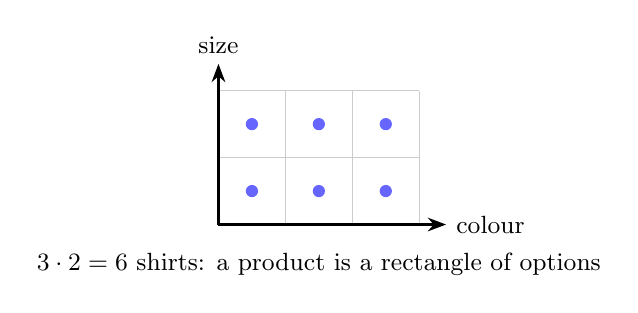
\begin{tikzpicture}[scale=0.85]
  \draw[step=1cm,gray!40,very thin] (0,0) grid (3,2);
  \draw[thick,-{Stealth}] (0,0) -- (3.4,0) node[right,font=\small]{colour};
  \draw[thick,-{Stealth}] (0,0) -- (0,2.4) node[above,font=\small]{size};
  \foreach \x in {0.5,1.5,2.5} \foreach \y in {0.5,1.5} \fill[blue!60] (\x,\y) circle (2.6pt);
  \node[font=\small] at (1.5,-0.6) {$3\cdot 2 = 6$ shirts: a product is a rectangle of options};
\end{tikzpicture}
\end{center}

\section{Products in the two \emph{Tárgytematika} documents}\label{sec:syllabi}

\subsection{Kalkulus I (MBLK37E)}

The syllabus text lists: \emph{A valós számtest.  Teljes indukció.  Nevezetes
egyenlőtlenségek.  Polinomok, racionális törtfüggvények, gyökös, trigonometrikus,
exponenciális függvények és inverzeik.  Értelmezési tartomány, értékkészlet, inverz
függvény, összetétel.  Grafikonok vázolása\dots{} Függvények határértéke\dots{} műveletek\dots{}
Elemi függvények deriváltja.  Láncszabály\dots}  The products hiding in it:

\begin{longtable}{@{}p{0.30\textwidth}p{0.14\textwidth}p{0.50\textwidth}@{}}
\toprule
\textbf{Syllabus item} & \textbf{Kind} & \textbf{Content, and the Lean name}\\
\midrule
\endhead
\emph{A valós számtest} --- the field $\mathbb{R}$ &
multiplication map &
The field operation is $m:\mathbb{R}\times\mathbb{R}\to\mathbb{R}$.  It is continuous
(\lean{mulMap\_continuous}) and bilinear (\lean{mulMap\_bilinear}), but \emph{not} linear
(\lean{mulMap\_not\_linear}).\\
\emph{Grafikonok vázolása} --- graphs &
product object &
A graph lives in $\mathbb{R}\times\mathbb{R}$; a curve $t\mapsto(f(t),g(t))$ is continuous
iff both coordinates are. \lean{top\_isProduct}\\
\emph{Értelmezési tartomány} of $f\pm g,\ f\cdot g$ &
product object &
The pairing $\langle f,g\rangle$ is defined on $\operatorname{dom}f\cap\operatorname{dom}g$:
intersection is the product taken inside the poset of subsets.\\
\emph{Határérték \dots műveletek} &
both &
$\lim (fg)=\lim f\cdot\lim g$ is exactly ``pair, then apply the continuous $m$''.
\lean{tendsto\_mul\_via\_product}\\
\emph{Elemi függvények deriváltja} (Leibniz rule) &
both &
$(fg)'=f'g+fg'$ is the chain rule for $m\circ\langle f,g\rangle$, with the derivative of
the bilinear $m$. \lean{product\_rule\_via\_product}\\
\emph{Összetétel}, \emph{láncszabály} &
neither! &
Composition is \emph{not} a product construction; it is the categorical composition.
Keeping $f\circ g$ and $f\cdot g$ apart is a graded skill.
\lean{comp\_ne\_pointwise\_mul}\\
\emph{Teljes indukció}, e.g.\ $n!<\big(\tfrac{n+1}{2}\big)^n$ &
multiplication map &
Iterated products; induction is how a statement about an $n$-fold product is reduced to a
binary one.\\
\emph{Exponenciális függvények és inverzeik} &
multiplication map &
$\exp$ converts $+$ into $\cdot$, $\log$ converts $\cdot$ into $+$: a homomorphism between
the two multiplication maps. \lean{log\_mulMap}\\
\bottomrule
\end{longtable}

\subsection{Lineáris algebra I (MBLK15E)}

The syllabus text lists, among others: \emph{Komplex számok\dots{} Vektorok és pontok a valós
elem-$n$-esek körében, vektorok összege és skalárral való szorzása\dots{} Belső szorzat,
vektorok hossza, háromszög-egyenlőtlenség, Cauchy--Schwarz-egyenlőtlenség\dots{}
Mátrixműveletek és azok algebrai szabályai\dots{} Mátrixegyenletek, mátrixok inverze\dots{}
Determinánsok\dots{} determinánsok szorzástétele, nemelfajuló mátrixok, Cramer-szabály.}

\begin{longtable}{@{}p{0.30\textwidth}p{0.14\textwidth}p{0.50\textwidth}@{}}
\toprule
\textbf{Syllabus item} & \textbf{Kind} & \textbf{Content, and the Lean name}\\
\midrule
\endhead
\emph{valós elem-$n$-esek} $\Rn$ &
product object &
$\Rn$ is the $n$-fold product of $\mathbb{R}$: a linear map into $\Rn$ is exactly its $n$
coordinate functionals, uniquely. \lean{pi\_isProduct}\\
Direct product $M\times N$ of spaces &
product object &
The product in the category of real vector spaces; a linear map into $M\times N$ is a pair
of linear maps. \lean{module\_isProduct}\\
\emph{skalárral való szorzás} $\mathbb{R}\times V\to V$ &
multiplication map &
Bilinear, defined on a product of two \emph{different} kinds of object.\\
\emph{Belső szorzat} $\langle u,v\rangle$ &
multiplication map &
$\Rn\times\Rn\to\mathbb{R}$, built coordinatewise out of the same $m$.
\lean{inner\_eq\_sum\_mulMap}\\
\emph{Mátrixműveletek}: $MN$ &
multiplication map &
Matrix multiplication is composition of linear maps: a map
$\mathrm{Mat}\times\mathrm{Mat}\to\mathrm{Mat}$. \lean{toLin\_matrix\_mul}\\
\emph{determinánsok szorzástétele} &
multiplication map &
$\det(MN)=\det M\cdot\det N$: $\det$ transports one multiplication map to the other.
\lean{det\_mul\_map}\\
\emph{mátrixok inverze}, \emph{Cramer-szabály} &
multiplication map &
Inverses are about the multiplication map, not the product object; the categorical
treatment is in \texttt{InverseOverlap.lean}.\\
\emph{Egyenesek, síkok, hipersíkok} &
product object &
A plane is a product of two lines; a linear system is read off coordinatewise, i.e.\ through
the projections of $\Rn$.\\
\emph{Komplex számok} $a+bi$ &
both &
$\mathbb{C}\cong\mathbb{R}\times\mathbb{R}$ \emph{as a product object} (real and imaginary
part), while complex multiplication is an extra bilinear map on it --- the same object
carrying both structures.\\
\bottomrule
\end{longtable}

\subsection{The overlap, in one sentence}

Both courses use the \emph{same} product object $\mathbb{R}\times\mathbb{R}$ and the
\emph{same} multiplication map $m$ on it; the two courses differ only in which property of
$m$ they exploit:

\begin{center}
\begin{tabular}{@{}lll@{}}
\toprule
\multicolumn{3}{@{}l}{One object $\mathbb{R}\times\mathbb{R}$, one arrow $m:\mathbb{R}\times\mathbb{R}\to\mathbb{R}$, two courses:}\\
\midrule
\emph{Kalkulus I} & $m$ is \textbf{continuous} &
  $\Longrightarrow\ \lim(fg)=\lim f\cdot\lim g$, $(fg)'=f'g+fg'$\\
\emph{Lineáris algebra I} & $m$ is \textbf{bilinear} &
  $\Longrightarrow\ \langle u,v\rangle$, $MN$, $\det(MN)=\det M\det N$\\
\bottomrule
\end{tabular}
\end{center}

\noindent
\lean{mulMap\_continuous\_and\_bilinear} records both at once.  And the reason
$(fg)'\neq f'g'$ --- the most common exam error --- is precisely
\lean{mulMap\_not\_linear}: $m$ is bilinear but \emph{not} linear, so it does not commute
with taking derivatives coordinatewise.

\section{Products and multiplication maps in \texttt{kalkulus\_gyakorlo.pdf}}\label{sec:atlas}

\begin{longtable}{@{}p{0.10\textwidth}p{0.40\textwidth}p{0.44\textwidth}@{}}
\toprule
\textbf{Exercise} & \textbf{What it asks} & \textbf{Product structure to use}\\
\midrule
\endhead
1.4 d) & Bound $\{p/q: p\in\{1,2,3,4\},\ q\in\{101,\dots,104\}\}$ &
The index set is a product of two $4$-element sets, so at most $16$ values; the bounds are
$\min/\max$ over a rectangle. \lean{exercise\_1\_4d\_card\_le}\\
1.12 & Inequalities such as $\frac{(x-3)(x+2)}{(x-4)(x-8)}<0$ &
A sign line is the statement that the sign map
$\{\pm\}\times\{\pm\}\to\{\pm\}$ is the multiplication map of signs; solve factor by factor
and multiply.\\
1.13 & $|a_1+\dots+a_n|\le|a_1|+\dots+|a_n|$ &
$|xy|=|x||y|$: the absolute value is a homomorphism for $m$ (proved in
\texttt{TriangleOverlap.lean}).\\
1.14 c) & $\sum_{i} q^i=\frac{q^{n+1}-1}{q-1}$ &
Telescoping after multiplying by $(q-1)$: the trick is to \emph{apply} a multiplication map
to the whole identity.\\
1.15 a), b) & $\sum i(3i+1)$, $\sum i(i+1)$ &
Each summand is a value of $m$ on a pair; expand by bilinearity, then use $\sum i$,
$\sum i^2$.\\
1.19 b) & Binomial theorem &
$(a+b)^n$ is an $n$-fold product; expanding it is choosing, for each factor, $a$ or $b$ ---
a product of $n$ two-element sets, so $2^n$ terms.\\
2.10, 2.12--2.15 & $f\circ g$, tables, equations &
\emph{Composition}, not product.  The exercise trains exactly the distinction of
Section~\ref{sec:test}. \lean{comp\_ne\_pointwise\_mul}\\
2.13 a) & $f(x)=x\sin x$ &
$m\circ\langle \mathrm{id},\sin\rangle$; differentiate with the Leibniz rule.
\lean{exercise\_2\_13a\_deriv}\\
2.17 a), b) & Are $f+g$, $f\cdot g$ injective? &
\textbf{No} in both cases: $m$ itself is not injective, and no hypothesis on the factors
repairs that.  Counterexamples $\mathrm{id}\cdot\mathrm{id}=x^2$ and
$\mathrm{id}+(-\mathrm{id})=0$. \lean{exercise\_2\_17b}, \lean{exercise\_2\_17a}\\
2.18 & $f\circ g$ injective if $f,g$ are &
\textbf{Yes} --- composition preserves monomorphisms, products do not.  Compare with 2.17
to see the difference between the two operations.\\
2.19 & A degree-$n$ polynomial has $\le n$ roots &
A polynomial is a product of linear factors over its roots; the multiplication map is
zero-divisor-free in $\mathbb{R}$.\\
3.2--3.4 & Limits of rational functions &
Factor, i.e.\ write the expression as $m\circ\langle\cdot,\cdot\rangle$, and use the product
rule for limits. \lean{tendsto\_mul\_via\_product}\\
3.7 & $\lim\frac{\sin 3x}{x}$, $\lim\frac{\tan 2x}{x}$, \dots &
Rewrite as a product of a known limit and a bounded/convergent factor, then multiply the
limits.\\
3.9 & One-sided limits of products/quotients &
The sign of the product is the product of the signs; the finite factor multiplies the
infinite one.\\
3.10 & $\lim(1+\tfrac{a}{x})^{x}$ &
An exponent is an iterated product: take $\log$ to convert it into a product, then into a
$\frac{0}{0}$ limit. \lean{log\_mulMap}\\
4.1--4.2 & Differentiate $x^5 5^x$, $x\cos^3 x$, \dots &
Every one of these is $m\circ\langle f,g\rangle$; apply the Leibniz rule.
\lean{product\_rule\_via\_product}\\
4.3 & Logarithmic differentiation, e.g.\ $\big(\tfrac{(x+1)(x-1)}{(x-2)(x+3)}\big)^5$ &
$\log$ turns a product into a sum, differentiate the sum, multiply back.  The whole method
is ``move along the homomorphism $\log$''. \lean{log\_mulMap}\\
4.11 a) & Split $20$ so that the product is maximal &
Maximise $m$ restricted to the line $x+y=20$: the answer is $10\cdot 10=100$.
\lean{exercise\_4\_11a}, \lean{exercise\_4\_11a\_attained}\\
4.12, 4.14, 4.15 & Area/perimeter optimisation &
Area is a multiplication map of two side lengths, constrained by a linear condition ---
the same shape of problem as 4.11.\\
\bottomrule
\end{longtable}

\section{Using the concept in a timed exam}\label{sec:exam}

\subsection{A four-step protocol}

\begin{enumerate}[label=\textbf{Step \arabic*.},leftmargin=2.2cm]
\item \textbf{Name the szorzat.}  Ask: is this a \emph{pair} (product object) or a
      \emph{value} (multiplication map)?  Write the answer in the margin: ``$\times$''
      or ``$m$''.  Ten seconds, and it selects the toolbox.
\item \textbf{Split.}  If it is a value $F=f\cdot g$, write $F=m\circ\langle f,g\rangle$ ---
      in practice, box $f$ and $g$ separately.  If it is a pair, handle the two coordinates
      separately: everything about a map \emph{into} a product is coordinatewise.
\item \textbf{Apply the property of $m$ that the question needs.}
      \begin{itemize}[nosep]
      \item Limit? Use continuity of $m$: $\lim(fg)=\lim f\cdot\lim g$ --- but only when both
            factors have finite limits.
      \item Derivative? Use bilinearity of $m$: $(fg)'=f'g+fg'$.
      \item Sign or inequality? Use that $m$ preserves the order in each variable separately
            when the other factor is $\ge 0$.
      \item Equation $=0$? Use that $\mathbb{R}$ has no zero divisors: $fg=0 \iff f=0$ or
            $g=0$.
      \item Too many factors? Take $\log$ and work with a sum.
      \end{itemize}
\item \textbf{Reassemble and check one number.}  Substitute a convenient value
      ($x=0$, $x=1$) into your answer and into the original.  Ten seconds, and it catches
      the common slips.
\end{enumerate}

\subsection{Four worked answers, in exam format}

\paragraph{(a) Exercise 4.2, differentiate $x^5 5^x$.}
Step 1: value, so $m$.  Step 2: $f=x^5$, $g=5^x$.  Step 3: Leibniz,
\[
  (x^5 5^x)' = 5x^4\,5^x + x^5\,5^x\ln 5 = x^4 5^x(5+x\ln 5).
\]
Step 4: at $x=0$ the function is $0$ with a fifth-order zero, and the answer vanishes
there. \hfill\lean{product\_rule\_via\_product}

\paragraph{(b) Exercise 3.7 b), $\lim_{x\to0}\frac{\sin 3x}{x}$.}
Step 1: value.  Step 2: $\frac{\sin 3x}{x}=\underbrace{\frac{\sin 3x}{3x}}_{\to 1}\cdot 3$.
Step 3: both factors have finite limits, so multiply them: the limit is $3$.
Step 4: for $x=0.01$ the quotient is $\approx 2.9996$. \hfill\lean{tendsto\_mul\_via\_product}

\paragraph{(c) Exercise 2.17 b), is $f\cdot g$ injective for injective $f,g$?}
Step 1: value.  Step 2: the composite $m\circ\langle f,g\rangle$ can only be injective if
$m$ separates the pairs that $\langle f,g\rangle$ produces --- and $m$ is very far from
injective.  Step 3: exhibit one counterexample, which is all an exam needs:
$f=g=\mathrm{id}$ gives $x^2$, and $1\neq-1$ while $1^2=(-1)^2$.  Answer: \textbf{no}.
Compare 2.18: for $f\circ g$ the answer is \emph{yes}, because composition, unlike $m$,
preserves injectivity. \hfill\lean{exercise\_2\_17b}

\paragraph{(d) Exercise 4.11 a), split $20$ so that the product is maximal.}
Step 1: it is a multiplication map restricted to a line --- a map out of a product,
constrained.  Step 2: eliminate one coordinate, $y=20-x$, i.e.\ parametrise the line by a
single variable; the object to maximise is $P(x)=x(20-x)$.  Step 3: $P'(x)=20-2x=0$ gives
$x=10$, and $P''=-2<0$, so $x=y=10$, $P=100$.  Step 4: $9\cdot 11=99<100$.  A one-line
alternative without calculus: $xy=100-(x-10)^2\le100$. \hfill\lean{exercise\_4\_11a}

\subsection{A time budget for a 90-minute paper}

\begin{center}
\begin{tabular}{@{}llp{0.46\textwidth}@{}}
\toprule
\textbf{Minutes} & \textbf{Phase} & \textbf{What products buy you}\\
\midrule
0--5 & Triage & Mark every ``$\cdot$'' in the paper as $\times$ (pair) or $m$ (value).
  The $m$-items are usually the fastest marks.\\
5--30 & Routine differentiation/limits & Leibniz and the product limit law, mechanically;
  do not re-derive them.\\
30--60 & Multi-step items & Logarithmic differentiation, factorised sign analysis,
  optimisation of an area.\\
60--80 & Conceptual items & Injectivity/surjectivity of $f\cdot g$ versus $f\circ g$;
  counting arguments; ``is this set a product?''\\
80--90 & Checks & Substitute one value in each answer; verify each ``product'' claim by the
  test of Definition~\ref{def:prod}.\\
\bottomrule
\end{tabular}
\end{center}

\subsection{Five traps that cost marks}

\begin{enumerate}[nosep]
\item \textbf{$(fg)'=f'g'$.}  False; $m$ is bilinear, not linear
      (\lean{mulMap\_not\_linear}).  The correct rule has two terms.
\item \textbf{$\lim(fg)=\lim f\cdot\lim g$ applied when one factor has no finite limit.}
      The hypothesis of \lean{tendsto\_mul\_via\_product} is that \emph{both} limits exist
      and are finite.  For $0\cdot\infty$ rewrite first.
\item \textbf{Confusing $f\circ g$ with $f\cdot g$.}  Different operations with different
      preservation properties: composition preserves injectivity (2.18), pointwise product
      does not (2.17 b).
\item \textbf{Assuming a constrained set of pairs is a product.}  ``All $(x,y)$ with
      $x+y=20$'' is a subobject of $\mathbb{R}\times\mathbb{R}$, not a product ---
      that is exactly why 4.11 is an optimisation problem and not a two-line calculation.
\item \textbf{Adding when the structure multiplies (or the reverse).}  Independent choices
      multiply (\lean{card\_prod\_eq\_mul}); alternatives add.  Deciding which one applies
      is Step~1 of the protocol.
\end{enumerate}

\subsection{The one-line summary to memorise}

\begin{center}
\fbox{\parbox{0.9\textwidth}{\centering
A \emph{product object} is a pair: maps \emph{into} it are handled coordinatewise.\\
A \emph{multiplication map} is an arrow out of a pair: it is continuous (so limits pass
through) and bilinear (so derivatives obey Leibniz), but it is neither linear nor injective.}}
\end{center}

\end{document}
